%!TEX root = mainfile.tex

\section{Observational Methods} % (fold)
% \label{sub:determingin_redshift}
	In this section we will outline 5 techniques considered for observing the EoR; the \SI{21}{\centi\metre} Line, CMB Anisotropy, Spectroscopy, Gravitational Lensing and the Dropout Method. Following a brief discussion of how they each work and the advantages and disadvantages of each, the justification for the selection of the techniques that will be employed is given.

	\subsection{Photometry and the Dropout Technique} % (fold)
		\label{ssub:filters_and_the_dropout_technique}
		(Dorothy, except~\ref{ssub:photometry} Joe)

		\subsubsection{Photometry} % (fold)
		\label{ssub:photometry}
			Photometry is one of the methods that astronomers use to detect objects in the universe. In principle, Photometry is the measurement of flux from objects through filters with a certain wavelength range (bandpass). These set of filters are known as a photometric system. There are three main types of photometric systems: Wide, intermediate and narrowband. As a rough guide for the visible band, wide filters tend to have bandwidth of 100nm, intermediate filters range from around 10 to \SI{50}{\nano\metre} and narrow bands range from 0.05 to \SI{10}{\nano\metre}\cite{Kitchin}. Photometry can often be confused with imaging, as it appears to be just imaging using a set of filters; astrophysicists take the view that Photometry is for the purpose of measuring the brightness of an object or objects in different wavelength bands and imaging is used to determine the structure and appearance of the object\cite{Kitchin}. Using a filter does not disperse the light as in spectroscopy, so if you use a filter with a large bandpass, more light is obtained in the image than if the observation was done using spectroscopy or narrow band filters. This means much fainter objects can be observed quicker using wide band photometry, this means it is a very effective method for studying many objects\cite{Romanishin}.
		% subsubsection photometry (end)

		\subsubsection{Dropout Technique} % (fold)
		\label{ssub:dropout_technique}
			Using photometry, the redshift of a LBG can be estimated using the dropout technique: The flux from the galaxy can be measured in three different bands, ideally two above and one below the Lyman break. If the galaxy is a high redshift Lyman break galaxy, it would be expected that, so long as the filters were correct for the redshift expected, one image would not see the galaxy whereas the other two would observe flux. Figure~\ref{fig:drop_out_at_z7} shows the dropout technique for a model galaxy of redshift seven.
			\begin{figure}[htbp]
				\centering
				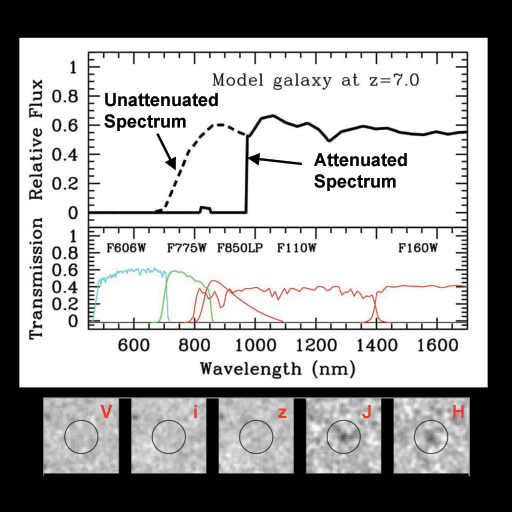
\includegraphics[width=0.5\textwidth]{../Images/drop_out_at_z7.png}
				\caption{Dropout technique for model redshift 7 galaxy\cite{first_galaxies_dropout_at_z7}.\label{fig:drop_out_at_z7}}
			\end{figure}

			The neutral hydrogen has attenuated almost all flux at wavelengths shorter than approximately 1 micrometre. The galaxy has been imaged in several different bands, and the longer wavelength filters show flux, whereas those at wavelengths corresponding to blueward of Lyman alpha do not. The galaxies that the group look to study have been shifted such that the drop happens in the infrared. The wavelength of the drop can be worked out using the known rest wavelength of Lyman alpha, as well as the factor by which the wavelength shifts due to the expansion of the universe, as shown in equation~(\ref{eq:dropout_wavelength}).
			\begin{align}
				1+z &= \frac{\lambda_{\text{observed}}}{\lambda_{\text{emitted}}}\label{eq:dropout_wavelength}
			\end{align}

			Since the rest wavelength of Lyman alpha is known and the observed wavelength of the drop can be measured, the redshift of the galaxy can be determined. This
			is only a rough estimate when doing photometry since the flux is simply a number in each of the bands. For example, if the bands do not overlap, and the drop happens between two bands, it will not be known at what point the drop occurred, only the range in which it occurred. This motivates the use of bands which are close together or potentially even overlapping. Figure~\ref{fig:filter-systems} shows some different bands and their bandwidth, for different filter systems. Johnson-Cousins- Glass is one of the oldest and still the most commonly used system\cite{BasicObservationalKnowledge}.
			\begin{figure}[htbp]
				\centering
				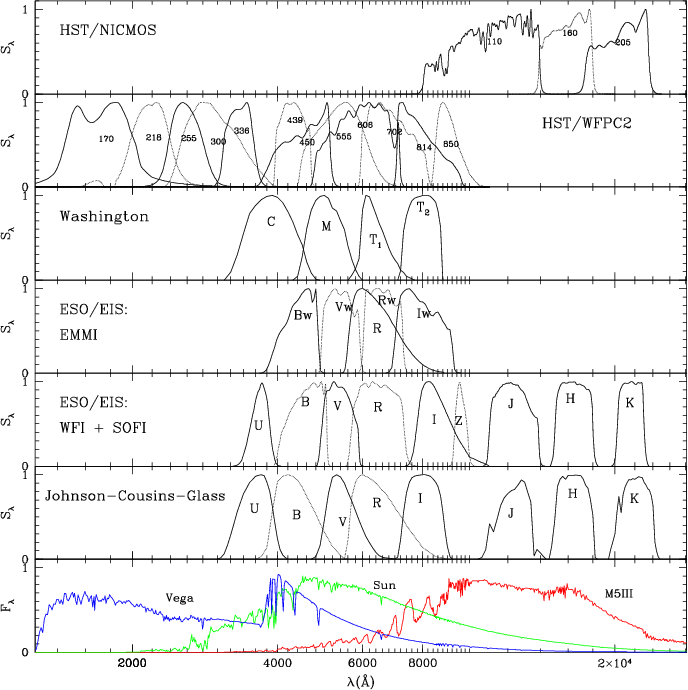
\includegraphics[width=0.65\textwidth]{../Images/filter-systems.png}
				\caption{Various filtering systems\cite{refId0}.\label{fig:filter-systems}}
			\end{figure}

			The bandpass is the wavelength range that can pass through the filter. Filters in different parts of the spectrum are given a common name, for example I band at \SI{806}{\nano\metre}. When observing LBGs, it is beneficial to have three filters in a row so that the position of the drop can be more accurately measured. As can be seen, there are gaps between the J H and K filters, meaning if the drop occurs between J and H, full flux should be observed in H and K and virtually no flux should be seen in J. (the panels beneath Figure~\ref{fig:filter-systems} show an image (or lack thereof) of the $z=7$ galaxy in each of the v, i, z, J and H bands)

			Table~\ref{tab:filter_characteristics} shows a list of filter names, the central wavelength of that filter, the bandwidth the filter covers, and range of redshifts for which the Lyman alpha drop would be covered. (This  range assumes the bandwidth covers 50\% either side of the central wavelength)
			\begin{table}[htbp]
				\begin{center}
					\begin{tabular}{c|c|c|c}
						Filter 	& Central wavelength & Bandwidth & Redshift coverage \\
						\hline \hline
						v 	& \SI{551}{\nano\metre}	 & \SI{88}{\nano\metre} & 3.17--3.90 \\
						i 	& \SI{806}{\nano\metre}	 & \SI{149}{\nano\metre} & 5.01--7.25 \\
						Y 	& \SI{1020}{\nano\metre} & \SI{120}{\nano\metre} & 6.90--7.88 \\
						J 	& \SI{1220}{\nano\metre} & \SI{213}{\nano\metre} & 9.16--9.91 \\
						H 	& \SI{1630}{\nano\metre} & \SI{307}{\nano\metre} & 11.14--13.67 \\
						K 	& \SI{2190}{\nano\metre} & \SI{390}{\nano\metre} & 15.41--18.61
					\end{tabular}
				\end{center}
				\caption{Data highlighting which filters would be useful for observing particular redshift galaxies\cite{Galactic_Astronomy_Binney_Merrifield}}
				\label{tab:filter_characteristics}
			\end{table}

			It must be taken into consideration that two filters should be redward of the drop and one blueward. One the fluxes have been measured in all three bands, if the object is indeed a LBG, there should be a sharp drop in flux in  one of the bands. However this does not totally rule out other possibilities: Some other objects could also exhibit a drop in flux, posing as LBGs, so usually a follow up method is used, and this is spectroscopy. 
		% subsubsection dropout_technique (end)
	% subsection filters_and_the_dropout_technique (end)

% subsection determining_redshift (end)
